\section{Pooling Layer}
\label{sec:pool_layer}

Convolutional layers can generate outputs that are bigger than the original input by computing a high number of filters.
Pooling layers are commonly inserted in-between successive Convolutional layers to progressively reduce the spatial size of the representation, in order to reduce the amount of parameters and computation in the network.

A Pooling layer re-sizes the input spatially, while it does not change its depth.
As for the case of the Convolutional layer, a patch is moved around the input and some aggregation function is computed to reduce the inputs to a single value.
The most common operator is the max function, even though other operations are possible \cite{CS231n}.

A Pooling layer requires to set some hyperparameters:
\begin{itemize}
    \item{\textbf{Spatial Extent}, which determines the dimension of the patch used to compute the aggregation function on the input image (similarly to the Receptive Field for Convolutional layers).}
    \item{\textbf{Stride}, which determines the amount of pixel the patch is moved on the image each time.}
\end{itemize}
A typical setting is to use max pooling with a spatial extent of 2x2 pixels and stride of 2, as shown in \cref{fig:pooling}.

\begin{figure}[ht]
	\centering
	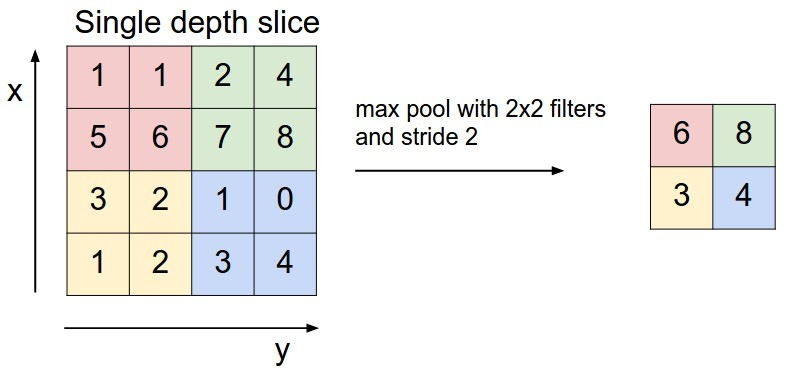
\includegraphics[scale=0.30]{figures/pooling}
	\caption{Illustration\protect\footnotemark ~of the pooling process. In this example, a patch of size 2x2 pixel is moved of 2 pixel at a time. The value computed is the maximum between the current values of the patch.}
	\label{fig:pooling}
\end{figure}
\footnotetext{Illustration taken from  \url{https://cs231n.github.io/convolutional-networks/}}
